%+++++++++++++++++ April
	\section{Introduction}
	
	
In this study, two different SEA designs have been implemented and tested. The first design is based on a linear movement (constrained by a linear guideway), where the rotary motion of the motor is driving a lever, pushing the carriage back and forth. For more details, see figure \ref{fig:actuation_system_explained}. \\
The second design is an approximated linear motion, due to a very large lever (rotational-L) actuated by a cam principle.
	
	\section{Design and Analysis}
	\subsection{Series Elastic Actuators}
	
		
	\subsection{Design of the PlayStation Controller}
	
	
	
	\subsubsection{Design of the Pilot Controller}
	
	
	
	\subsection{Test Environment and Programs}
	
	
	
	\subsection{Photoreceptor Circuit}
	The photoreceptor that has been used is the TPR-105 from GENIXTEK CORP. Its sensing characteristics can be seen in figure \ref{fig:photoreceptor_curve}. The electrical circuit can be seen in figure \ref{fig:tpr105_circuit}. The component values are $R_1 = 330 \Omega$, $R_2 = 62$k$\Omega$ and $V_{CC} = 5$V. This receptor returns a $10$-bit value.
	
	\begin{figure}[h!]
		\centering
		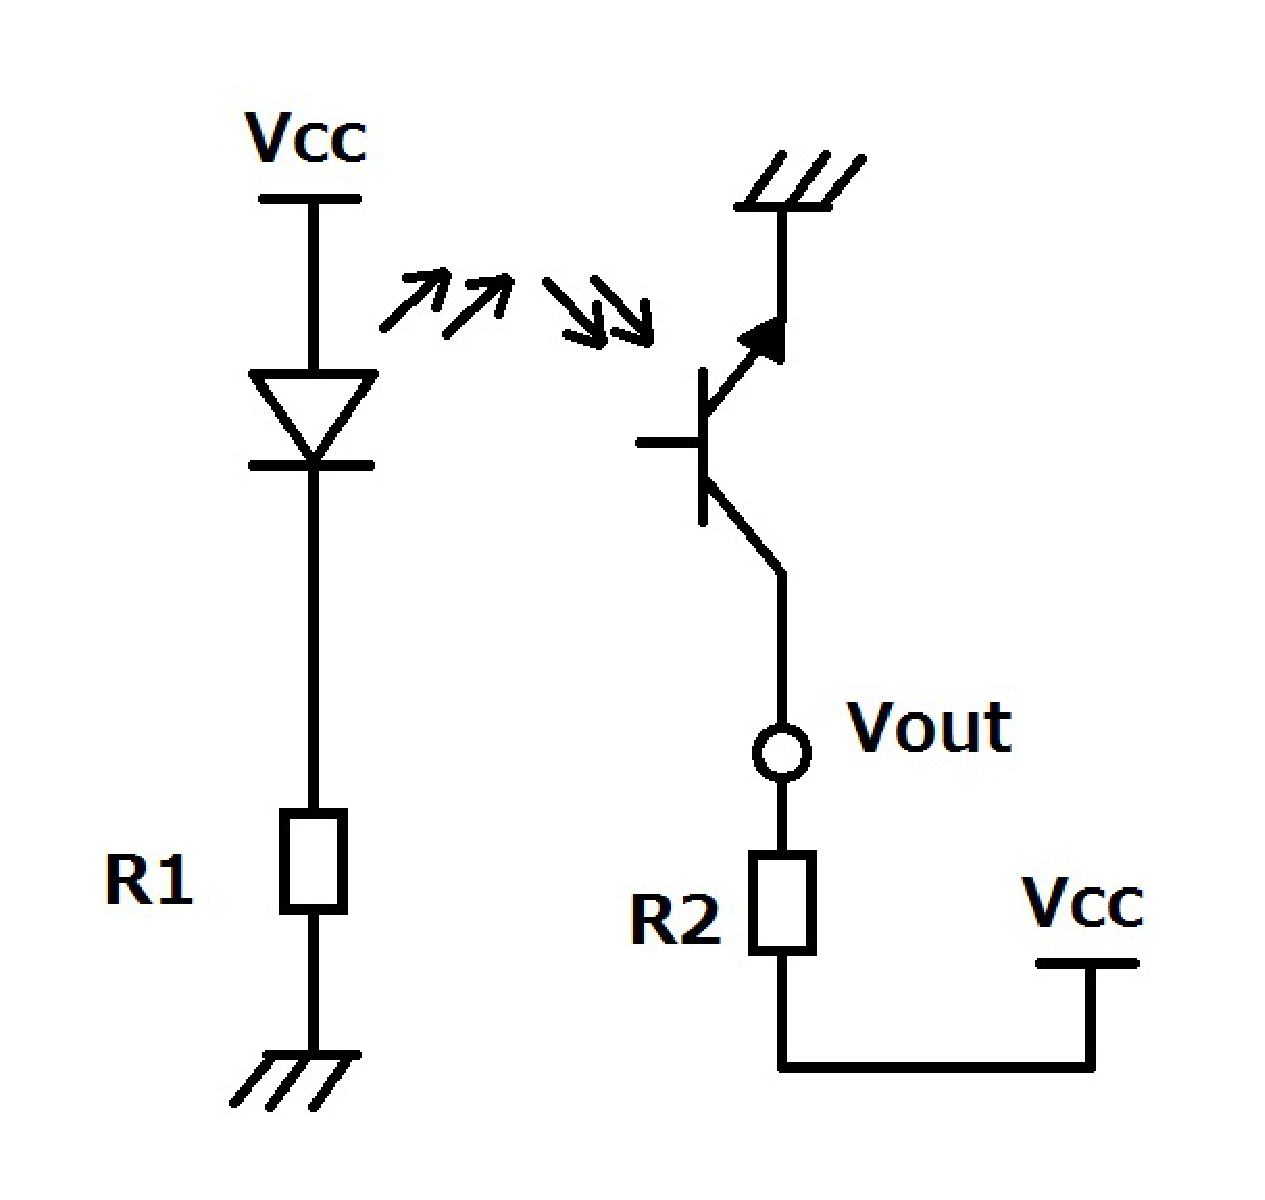
\includegraphics[width=0.2\linewidth]{Figs/tpr105_circuit}
		\caption{Implementation circuit of the photoreceptor.}
		\label{fig:tpr105_circuit}
	\end{figure}
	\begin{figure}[h!]
		\centering
		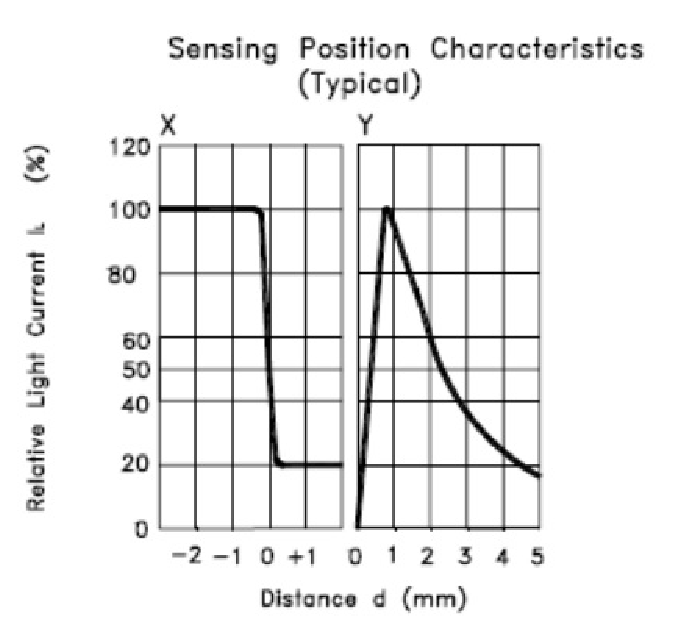
\includegraphics[width=0.3\linewidth]{Figs/photoreceptor_curve}
		\caption{Sensing characterstics of the photoreceptor TPR-105. Taken from its datasheet.}
		\label{fig:photoreceptor_curve}
	\end{figure}

	The sensing characteristics shows a nonlinear function in the range between $1$mm and $5$mm. However, as a first step, this has been interpolated linearly. To put it more precisely, the target output force has been mapped linearly to the measured distance. The operational distance lies between $4.5$mm to $5.5$mm.
	
	\section{Testing of the PlayStation Controller}
	For the two sides of the controller two different spring constants have been used. On the left-hand side, there is a set of three springs with a constant of $0.98$N/mm each. The motor has a reduction gear ratio of $33:1$. On the right-hand side the springs have a constant of $9.8 $N/mm and the motor has a reduction of $112:1$. The parameters are resumed in table \ref{tab:playstation_charac}.
	
	\begin{figure}[h!]
		\centering
		\begin{tabular}{|l|c|c|l|}
			\hline
			& Left side & Right side & Units\\ \hline \hline
			Clamp link length & 20 &  20 & [mm]  \\ \hline
			Motor reduction & $33:1$ & $112:1$ &  [-] \\ \hline
			Output torque (continous) & $30$ & $93$ & [mNm]  \\ \hline
			Output torque (intermittent) & $100$ & $180$ & [mNm] \\ \hline
			Number of springs used & $3$ & $3$ & [-] \\ \hline
			Spring constant & $0.9$ & $9.8$ & [N/mm] \\ \hline
			Equivalent spring constant & $2.7$ & $29.4$ & [N/mm] \\ \hline
		\end{tabular}
		\caption{Motor setup characteristics}
		\label{tab:playstation_charac}
	\end{figure}

	In order to conduct the frequency response analysis, the SG-4115 Function Generator has been used. The output signal was a sine wave with a peak-to-peak value of $2$V and an offset of $1.4$V. These settings have been made in order to stay within the detectable range of the Arduino $[0..5]$V. The frequency has been varied between $0.1$Hz and $35$Hz with $20$ logarithimcally spaced steps.
	
	Since the palm pads are blocked by the users hand in operational mode, they may not be considered blocked by an infinitely stiff wall. Therefore two different test setups have been created, where the palm pad has first been blocked by a screw driver in both directions, to have close to infinite stiffness, and a second setup, where the palm pads have been blocked by the users hands.
	
	\subsection{Results for Fixed Palm Pad Experiment (Pseudo Infinite Stiffness)}
	The input signal has been received as a feedback value (ie. $dist_{ref}$) and the P-controller stated in table \ref{tab:programming_params} controlled the output force by linearly mapping it to the photoreceptor distance. The measured distance has been logged and plotted. As it was expected, it is between the two extreme values stated in table \ref{tab:programming_params} (MIN and MAX). The response for the two extreme frequencies can be seen in figure \ref{fig:resp_left_hand_rigid_experim1}.
	\begin{figure}[h!]
		\centering
		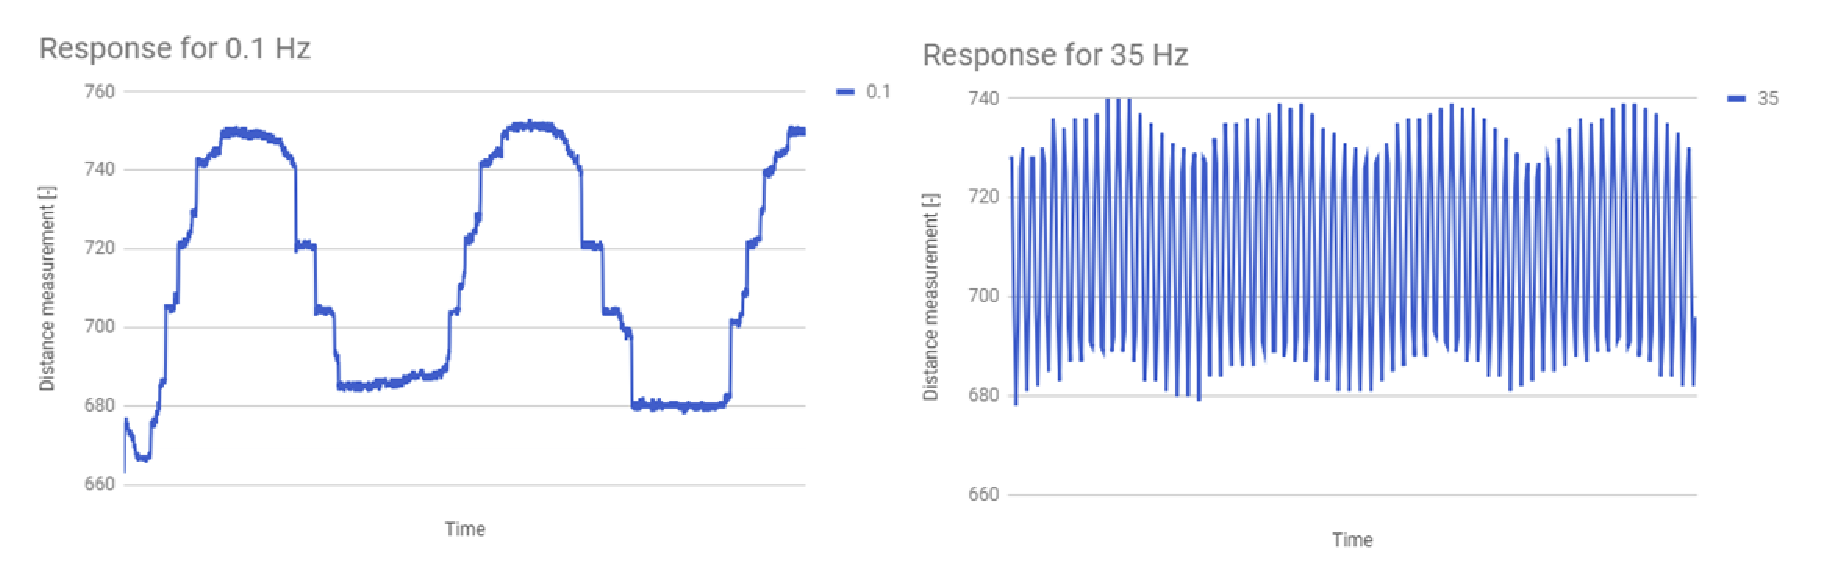
\includegraphics[width=0.7\linewidth]{Figs/resp_left_hand_rigid_experim1}
		\caption{}
		\label{fig:resp_left_hand_rigid_experim1}
	\end{figure}
	
	
	To calculate the amplitude of the output function (the measured value by the photoreceptor, corresponding to the distance between sensor and palm pad) one should ideally have a distinguishable value which is given by the maximal and minimal value of the sinusoidal output function. However, due to noise in the system, a sometimes occurring drift, interpolation aliasing and other effects such as the plateau characteristics shown in figure \ref{fig:resp_left_hand_rigid_experim1} and discussed in a later section, these minimum and maximum values are not clearly defined. Therefore, two different approaches have been chosen for the pseudo infinitely blocked palm pad experiment.
	
	First, the two quartile values ($Q_1$ and $Q_3$) have been calculated based on all the data, including outliers and noise. This is a relatively time-efficient method and is supposed to be less accurate since it sometimes includes errors such as the initial downward spike shown in the figure \ref{fig:resp_left_hand_rigid_experim1} for $0.1$Hz. The difference between these two quartile values has then been divided by the difference of the quartiles of the input signal ($Q_{3(sine)} - Q_{1(sine)}$). The results are indicated by the blue lines in figure \ref{fig:freq_resp_both_hands_rigid_experim1}.
	
	
	\begin{figure}[h!]
		\centering
		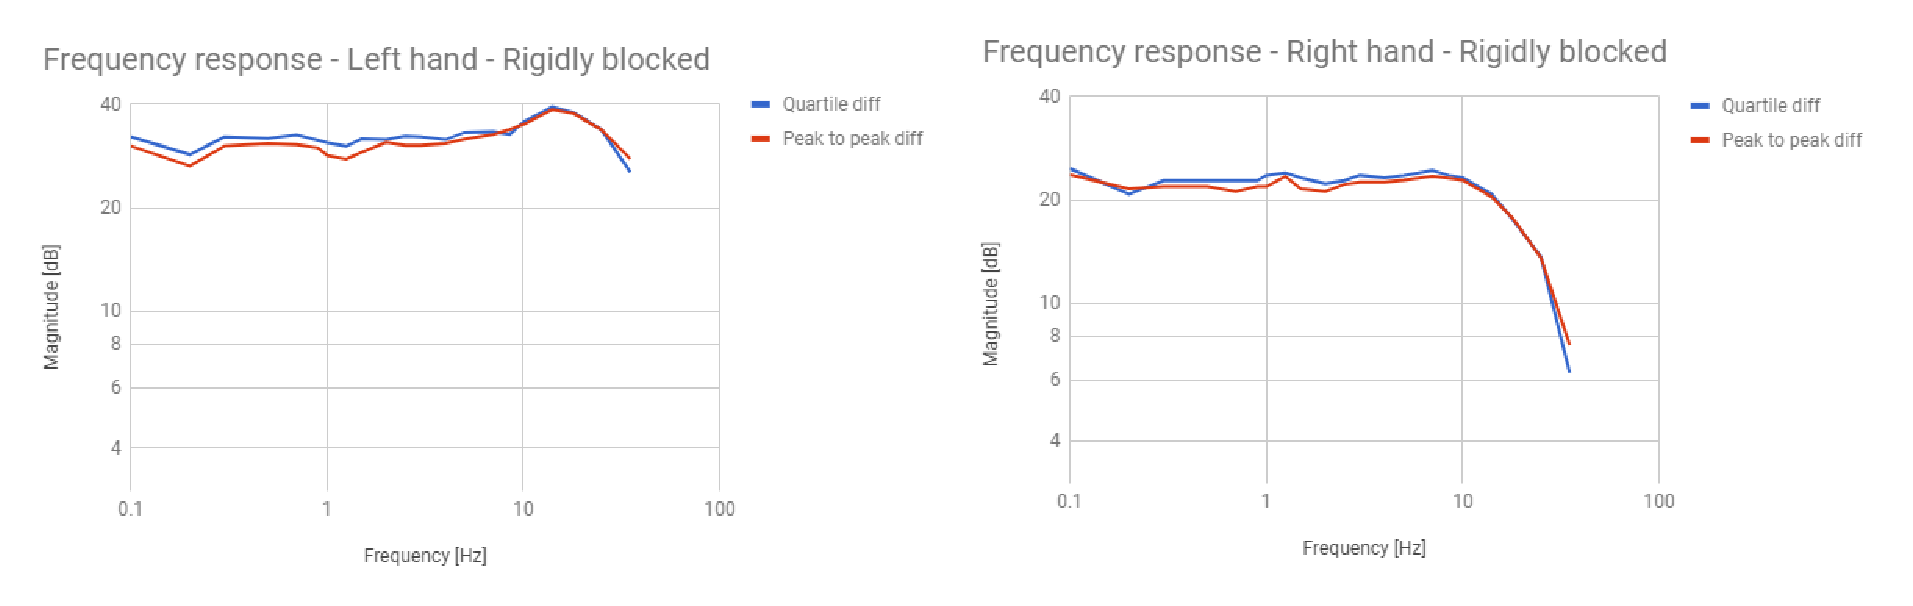
\includegraphics[width=1\linewidth]{Figs/freq_resp_both_hands_rigid_experim1}
		\caption{Frequency response analysis for both hands with a pseudo infinitely blocked palm pad.}
		\label{fig:freq_resp_both_hands_rigid_experim1}
	\end{figure}

	As an alternative output function, the amplitude has been measured manually, taking an average over several minima and maxima. This method is much more time consuming, but allows for filtering the noisy parts of the measurement, since it requires a visual representation of the measured data. These values are indicated on the same figure by the orange lines.
	
	\subsection{Results for Hand-Blocked Palm Pads Experiment}
	In the second experimental setup, the palm pads have been blocked by the hands of the user, to simulate an environment closer to the operational mode. This time, only the quartile method has been used to calculate the amplitude of the output signal. The results can be seen in figure \ref{fig:freq_resp_both_hands_soft_experim1}.
	\begin{figure}
		\centering
		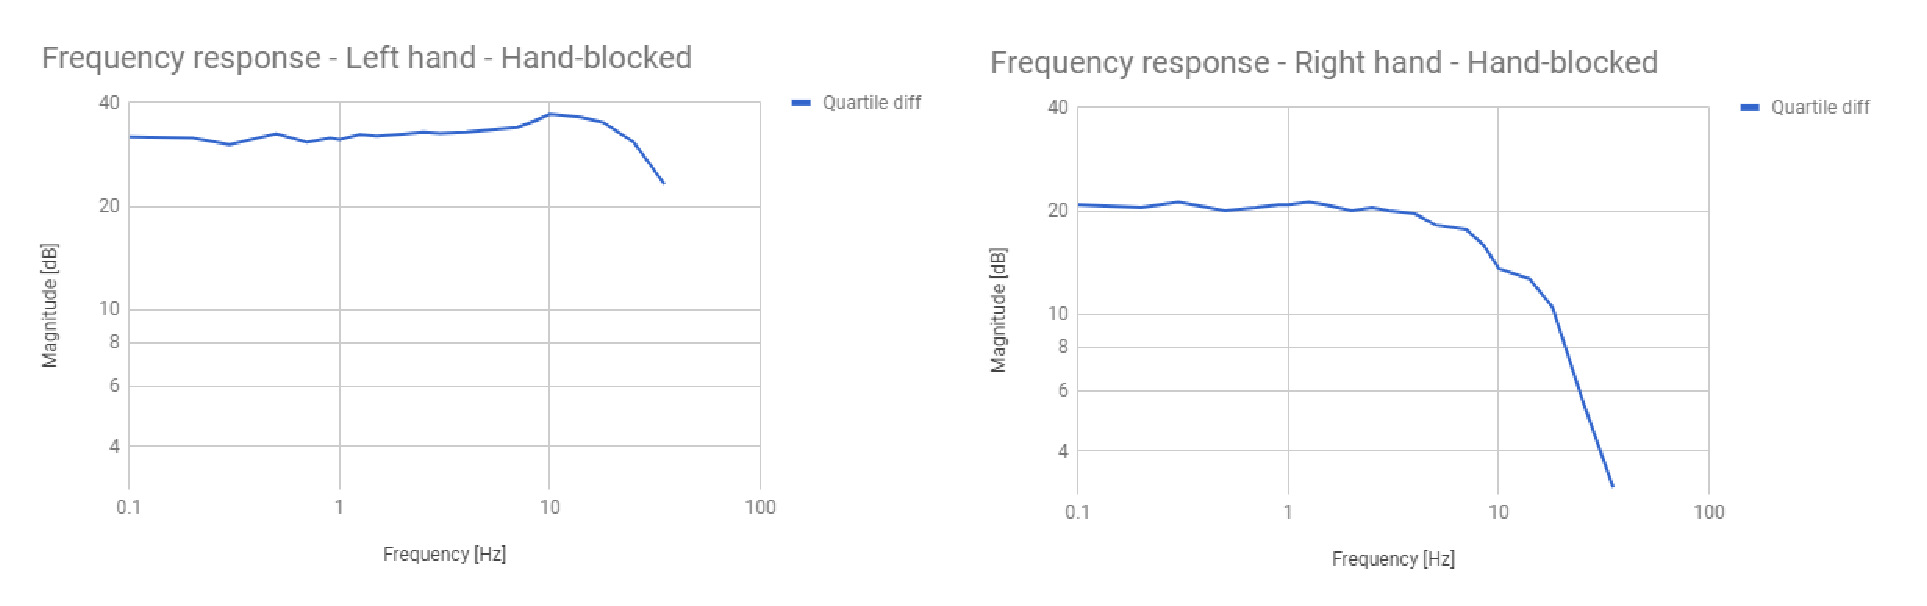
\includegraphics[width=1\linewidth]{Figs/freq_resp_both_hands_soft_experim1}
		\caption{Frequency response analysis for both hands with a hand-blocked palm pad.}
		\label{fig:freq_resp_both_hands_soft_experim1}
	\end{figure}
	
	The order of the system can be identified when looking at the slope of the Bode plot after its resonance top\footnote{Acutally, one should also consider the phase plot, but due to the reasons mentioned later in this research, this step has been skipped.}. This has been calculated for the six different curves and the following slopes have been found:
	
	\begin{tabular}{|c|c|c|}
		\hline 
		Rigid & left hand, blue line & $-54$ dB per dec \\ 
		\hline 
		& left hand, orange line & $-65$ dB per dec \\ 
		\hline 
		& right hand, blue line & $-54.8$ dB per dec \\ 
		\hline 
		& right hand, orange line & $-60.4$ dB per dec \\ 
		\hline 
		Soft & left hand & $-62.4$ dB per dec  \\ 
		\hline 
		& right hand & $-41.1$ dB per dec \\ 
		\hline 
	\end{tabular} 
	
	\section{Discussion}
	\subsection{Control Scheme and GUI}
	The control scheme is a simple proportional controller. It has been tested and decided to work well enough. If time permits, an integration and fine-tuning of an integral and derivative term can be done. \\
	There is not much to say about the GUI, however the handling of messages is not always done successfully. From time to time the processing program receives a message from the robot which is not complete. This results in accessing a cell of an array that is out of boundaries and the program crashes. To ensure the stability of the program, this case needs to be handled.
	
	\subsection{Design and Fabrication of the PlayStation Controller}
	The design of the controller is rather bulky and the actuation system might be too complex for what it is supposed to do. Due to its size, the upper and lower parts do not fit in the 3D printer and had to be cut in half and assembled by screws. This adds an extra step in manufacturing and assembly, making it more time-consuming. However the overall assembly is quite easy and tolerances have been chosen such that the whole system works. The feedback direction is not chosen optimally, if one aims at having a feedback opposing the driving direction (as seen from the robot).
	
	\subsection{Design and Fabrication of the Pilot Controller}
	This controller has almost been fully assembled, however not tested yet. It is much more simple to manufacture, as well as assemble. This design focused on having a feedback opposing the direction of motion.
	
	
	\subsection{Frequency Response Function}
	Figure \ref{fig:resp_left_hand_rigid_experim1} mainly shows two things. Firstly, there seems to be a certain step size, which is considerably more than expected. This results in only few values to attain for the photoeceptor, which can easily be seen in the response for $0.1$Hz. The second thing is, that at higher frequencies the Arduino has a too low update frequency and cannot follow the imposed sine signal, resulting in some aliasing effects. This shows that the Arduino is not capable of following frequencies higher than $35$Hz, but it also shows that the Arduino is not the right choice as a control device. The data analysis is therefore only to take with a grain of salt, since the important region after the resonance top had to be cut off. Future experiments shall be conducted using an mbed device, capable of operating at a control loop frequency of at least $1$kHz.
	
	As it can be seen in figure \ref{fig:freq_resp_both_hands_rigid_experim1} the two different methods of measuring the amplitude of the output signal share the same allures to a certain extent. This legitimizes to use the much more time-efficient approach of calculating the amplitude using the two quartile values. This argument has already been used for the data analysis in the experiment where the palm pads have been blocked by the users hand.
	
	The two figures \ref{fig:resp_left_hand_rigid_experim1} and \ref{fig:freq_resp_both_hands_rigid_experim1} show similar characteristics. Based on this, it seems appropriate to treat the two cases of pseudo infinite stiffness and hand-blocked palm pads as the same environment and for ease of analysis, only one of the two cases shall be treated.
	
	
	
	\section{Conclusion}
	The data that has been gathered with the Arduino as control device is only significant to a certain extent. The conclusions of using a screwdriver to block the palm pads for the experiments instead of the hand is still valid. However, the investigated frequency regions are too low to draw a meaningful conclusion and thus needs to be studied in more detail with a different control device (ie. an mbed). In addition to that, the phase diagrams have to be taken into account to confidently determine the order of the system.\\
	Furthermore, the most sensitive range of the photoreceptor is between $1$mm and $2$mm. The current implementation however is at a distance of roughly $5$mm making it much less linear and also less sensitive. This distance shall be reduced to increase linearity and sensitivity.
	
	
	\section{Outlook}
	First, the measured distance of the photoreceptor shall be changed to be in the range of $1.5$mm to $2.5$mm to have maximum linearity and sensitivity.\\
	The next step is to program the mbed to achieve the same control structure as with the Arduino, only with a higher control frequency. This should make it possible to study the system for higher frequencies. The control frequency shall be of $1$kHz, aiming for a maximum frequency of $100$Hz (Nyquist frequency is $f_s = 500$Hz and the practically achievable frequency is roughly one $5$th of this value).\\
	The experiments shall be conducted and analyzed again, this time also taking into account the phase plot in the Bode diagram. \\
	Additionally, the second controller shall be fully assembled and tested in the same manner.\\
	In parallel, the datasheet of the PMA servo motor driver shall be translated into English and the device integrated in the setup.

	
	%‚±‚±‚Ü‚Å
}










%+++++++++++++++++ May
	
	\section{Introduction}
	This report is the continuation of the first report about the project "Haptic Feedback Controller with Palm Pressurization". The last report has left off with the conclusion that the Arduino had a limited operating frequency and that the gathered data was not reliable enough, since not the whole region of interest in frequency could be covered. First, the idea was to use an mbed and program it to be able to replace the Arduino. However, with a few tricks %TODO explain what I did with prescaler and such
	it was possible to reduce the time of some commands to a minimum to stay at an operating frequency of $1$kHz. \\
	This report explains the setup and states the result for the adapted controller and provides a somewhat short explanation and discussion of the gathered data.
	
	\section{Experiment and Data Gathering}
	
	
	
	
	
	\subsection{Photoreceptor Circuit}
	
	
	\section{Frequency Response Analysis}
	To conduct the frequency response analysis in a meaningful environment, the controller has to be tested under conditions close to the operational ones. To be able to control the distance between the palm pads and the L-plates, and therefore the compression ratio of the springs, the palm pads have been blocked mechanically. With the wave generator producing the reference signal, the Arduino controlled the motors to match the compression with the reference. Figures \ref{fig:1plot_zoom} to \ref{fig:100plot_zoom} show some testcases.
	
	
	\begin{figure}[!htb]
		\minipage{0.32\textwidth}
		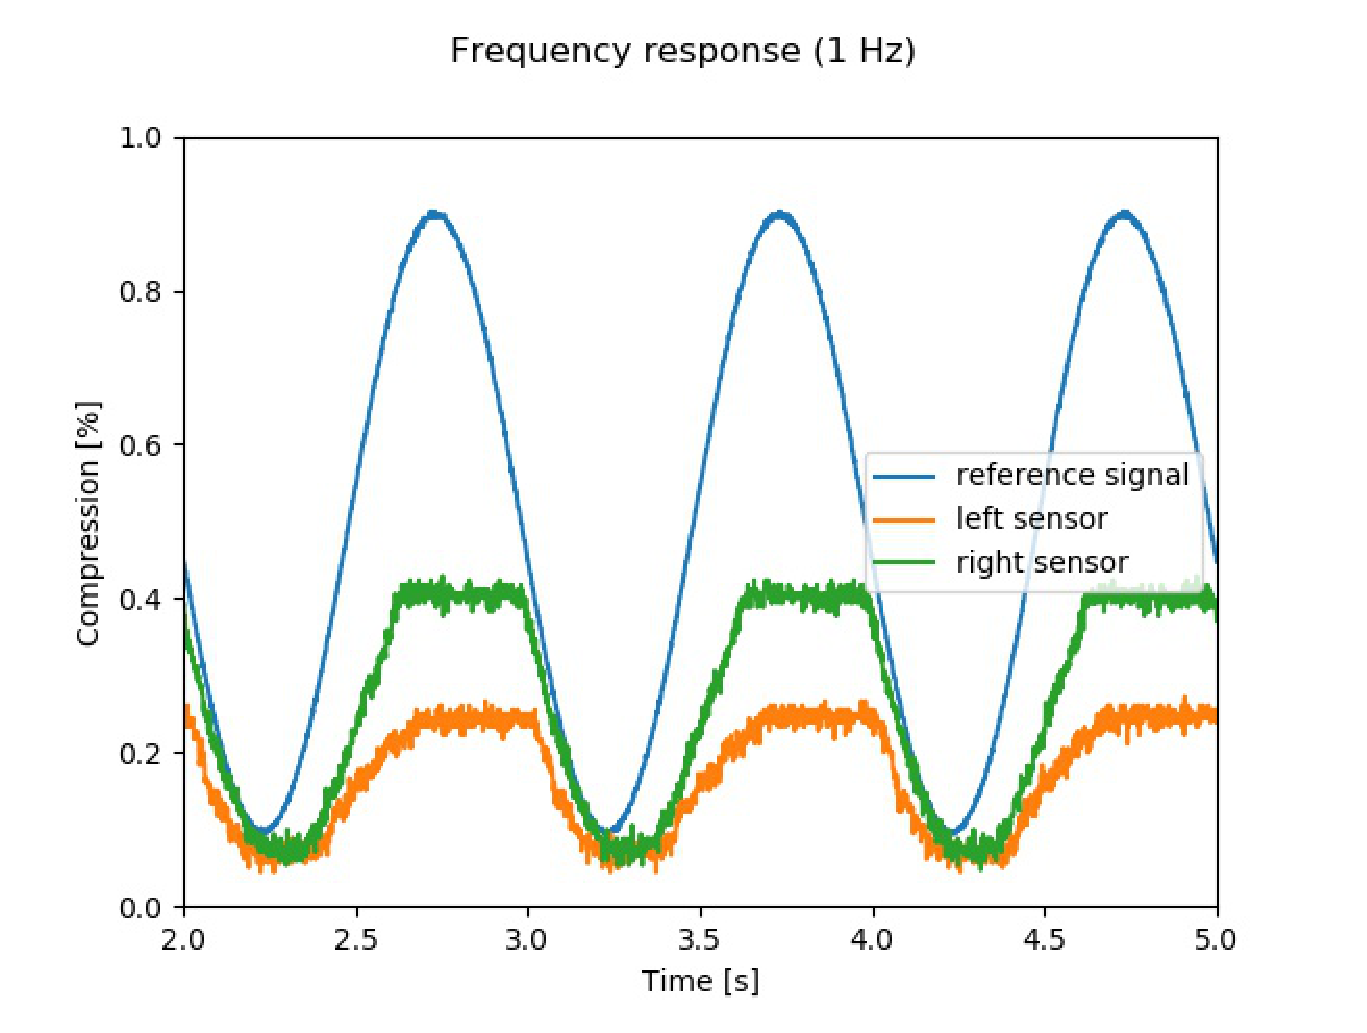
\includegraphics[width=\linewidth]{Figs/1plot_zoom}
		\caption{1 Hertz}\label{fig:1plot_zoom}
		\endminipage\hfill
		\minipage{0.32\textwidth}
		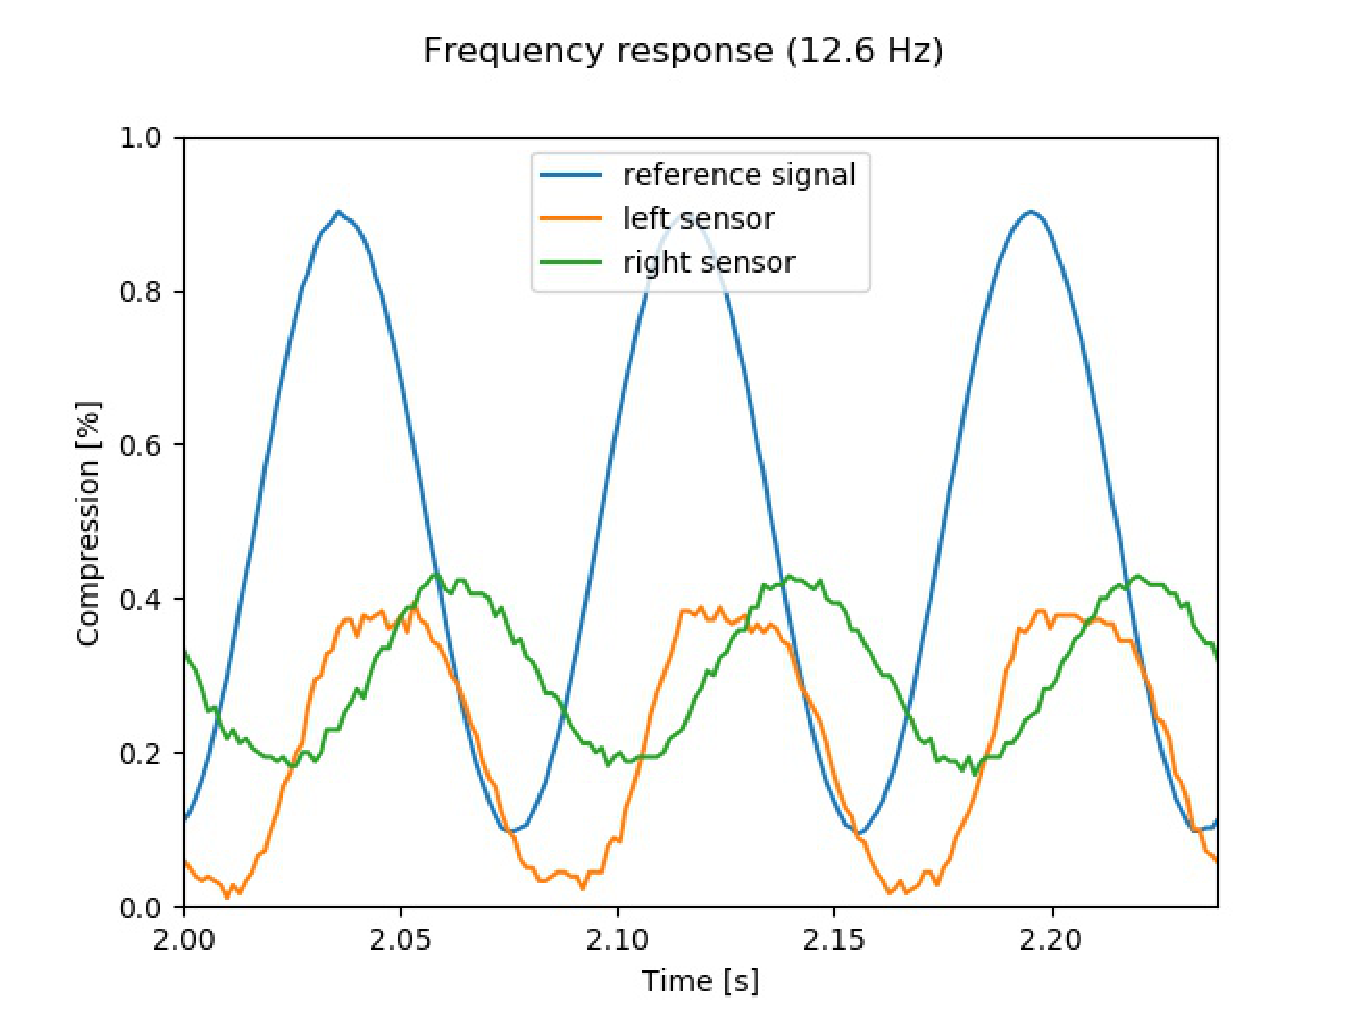
\includegraphics[width=\linewidth]{Figs/12.6plot_zoom.eps}
		\caption{12.6 Hertz}\label{fig:12.6plot_zoom}
		\endminipage\hfill
		\minipage{0.32\textwidth}%
		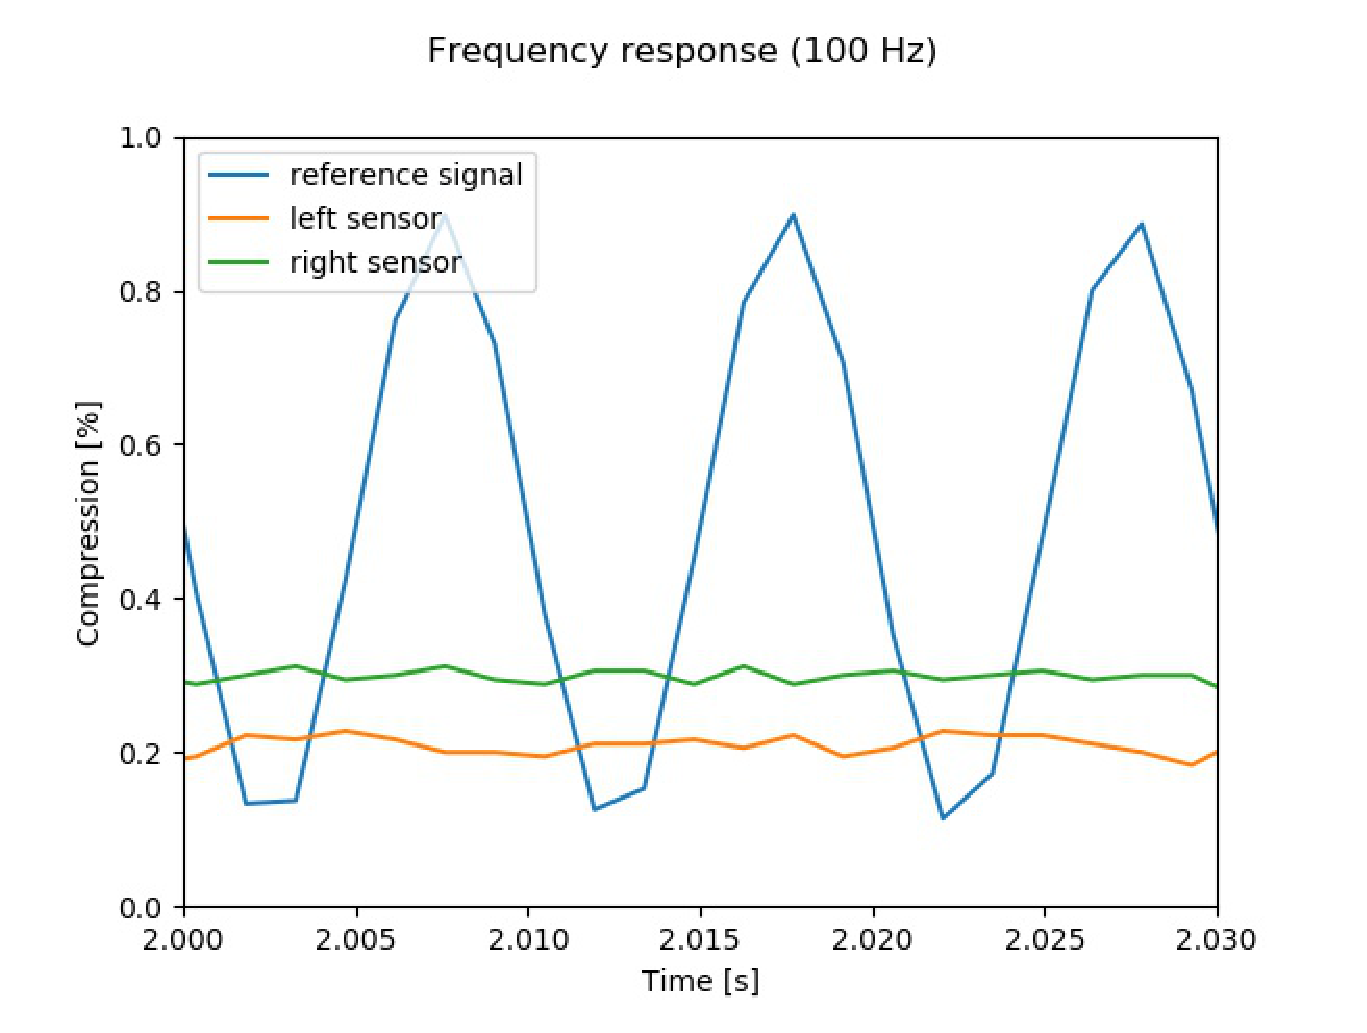
\includegraphics[width=\linewidth]{Figs/100plot_zoom}
		\caption{100 Hertz}\label{fig:100plot_zoom}
		\endminipage
	\end{figure}
	With these signals one can calculate the amplification factor between the reference signal and the output signal, as well as the phase shift.
	
	

	
	

	\section{Conclusion}
	The Bode diagrams show promising results. This is a first hint that the implementation of the series elastic actuators is not slowing down the system, since the bottleneck is given by the robot GUI communication link.\\
	
	\section{Outlook}
	The input signal is interfering with the output signal on the Arduino. Therefore it is necessary to investigate its impact by implementing a voltage follower to reduce the output impedance.\\
	A theoretical model shall be calculated to take into account the different aspects and parameters of the setup. The goal is to come up with a precise model to simulate different parameter settings, such as equivalent spring constant, motor parameters or operating frequency.
	

	
	%‚±‚±‚Ü‚Å
}










%+++++++++++++++++ June
	
	\section{Introduction}
	This report is the continuation of the first two reports about the project "Haptic Feedback Controller with Palm Pressurization". The last report has left off with the idea of implementing a voltage follower and suggested to retake measurements to create a Bode diagram. Furthermore, it has been suggested to create an analytical model and analysis of the setup in order to run simulations to identify setup parameters such as the equivalent spring constant, gain values or motor parameters.
	
	
	
	
	
	
	%show picture, explain problem of steady state offset, find PID values
	










\section{Discussion}
\subsection{P-controlled Device}
As figure \ref{fig:bode_sp_damp300_P02} indicates, the results of the mathematical model seems to correspond with the experimental data. Furthermore, a damping coefficient of $b_{sp} = 300$ Ns/m could be identified. The tracking behavior of this P-controller was reasonable for lower frequencies, even though there was a slight steady-state offset. The constant phase-lag was very small for small frequencies and did not exceed $45^\circ$ for frequencies up to $10$ Hz. Even an approach of discretizing the analytical results did not yield a better match of the results. %TODO necessary to discuss this, or show the graph?
 
\subsection{PID-controlled Device}
When the PID-controller has been implemented, the difference between analytical results and the experiments was much bigger. First it was noteworthy, that the two motors showed a different behavior with the same gains. This might stem from several asymmetries in the setup. First of all and most importantly, the distance sensors are different, and have different threshold values. Also, the springs might not have been glued in a perfectly symmetrical manner. However, the noise characteristics of the sensors are in a similar order of magnitude and do not account for the differences here. Lastly, there are the mechanical aspects of how the motors have been screwed to the controller. Due to the high-frequency driving, the screws loosen from time to time, which can have a significant impact on the Bode plots. Furthermore, there might be a slight misalignment of the motor shaft axis and the guideway, which results in an opposing force.\\
Again, the discretization of the analytical transfer function did not yield a better match between the analytical and experimental data.\\
Judging from the frequency response seen in figure \ref{fig:bode_sp_damp100_PID} the tracking is relatively bad at low frequencies, not only because there is an attenuation, but also that the resonance top at higher frequencies quickly leads to saturation of the applicable motor voltage. In addition to this, the phase lag is much bigger and is already at least $45 ^\circ$ in the lower range of the bandwidth. This is due to the filters that have been used. The first filter is an RC-circuit that takes the PWM signal from the arduino and produces a more continuous voltage signal for the amplifiers. The cut-off frequency is $330$ Hz. 

% talk about filter and filter impact, problem of discretization, results	

\section{Conclusion}
Given the results for the P-controller, one can assume that the mathematical model is correct. However, when one implements a PID-controller, a higher discrepancy between mathematical model and experimental data arises. Even though the parameters used in the mathematical model have been double-checked (such as the moment of inertia for example), its validity can be questioned.\\
From the two different implementations, the P-controller shows a better tracking behavior for the operational bandwidth.

\section{Outlook}
In the future, the P- and PID-controller shall be tested and a subjective measure of the feedbacks smoothness and transparency shall be reported.\\
A more thorough literature review shall be done to discuss the findings with existing papers.\\
A design-choice guide shall be created in order to facilitate future research for similar setups.


	
	%‚±‚±‚Ü‚Å
}









%+++++++++++++++++ July
	
\section{Introduction}
This report is the continuation of the first two reports about the project "Haptic Feedback Controller with Palm Pressurization". The last report has stated the tracking behavior of a simple P- and PID-controlled device for a sine reference of various frequencies. Furthermore, it has suggested an experimentally identified equivalent spring damping coefficient which can be used to model the setup analytically.\\
This report is first introducing a thorough literature research into the haptic teleoperated field of study. Then it will discuss the results of the tested controller and give advice on how to choose system and setup parameters for future and related work. 

\section{Project Introduction}


%Hannaford shows that a cable driven hand-controller has similar frequency characteristics, where the resonance frequency is slightly more elevated than the SEA device.

\section{PlayStation-Controller Testing}


\section{Design Framework}


\section{Pilot Controller}
Based on the framework from the previous section, a new controller has been devised, mainly focusing on a different design and on a more optimal feedback direction.

\subsection{Working Principle (cam)}%TODO put text from april here
Has already been stated in April's monthly report.


%state the parameter choices that i have made based on previous findings
\subsection{advantages and disadvantages}%TODO is this really necessary or can i write it under design and parameters
%state advantages and disadvantages
\subsection{Analytical results}
%state analytical results (if available)
\subsection{Frequency Response Analysis}
Similar to the previous frequency response analysis, the controller has been tested when feeding a sine wave in the range of $1$ Hz up to $100$ Hz. The result for the P-controlled device can be seen in figure \ref{fig:pilot_bode_P02}

\begin{figure}[h!]
	\centering
	\includegraphics[width=0.6\linewidth]{Figs/pilot_bode_P02}
	\caption{Frequency response function of the P-controlled pilot controller.}
	\label{fig:pilot_bode_P02}
\end{figure}

The bode diagram resembles the one of the previous setup, with the main difference, that it seems to be shifted towards lower frequencies. The phase offset changes almost linearly from $45 ^\circ$ to $200 ^\circ$. Analogously, it is argued that the initial phase lag for low frequencies stems from the different filters that have been implemented in the same manner. Regarding the magnitude plot however, it is important to note that the resonance frequency is much lower, namely $4$ Hz.\\

In the current design of the pilot controller, the lever is roughly $100$ mm and has been fabricated using an $8$ mm thick poly-acetal plate. Due to the relative low thickness, the lever can deform and thus leads to an additional spring element in the system. Furthermore, the rotation cam is not coupled to the lever and thus cannot make pull it back in order to decrease the springs' compression, even if a negative voltage is applied. This leads to a lower overall performance and results in a lower resonance frequency.\\
In order to deal with this issue, it is recommended to preload the lever that pulls it back faster than normal, or couple the rotational cam with the lever.

\subsection{Pilot-Controller Testing}
%state real feel, latency, transparency and stability
\subsection{Outlook}
%state possible improvements for future work


\section{Discussion}	

\section{Conclusion}


\section{Outlook}



	
	%‚±‚±‚Ü‚Å
}

